\section{Application on an Airfoil}

The goal of this part was to use the previous functions to demonstrate the flow and behavior of
air around the airfoils of an airplane. In other words, showing how air moves around airfoils in order to produce that
lift force and as little air turbulence as possible. Moreover, the aim was to draw the pressure map that
the airfoils were going to be put under in order to deduce information like the maximum pressure
a wing can handle and which parts can handle more or less pressure.

\subsection{Modeling the Airflow }

An airfoil is supposed to operate in a laminar flow, which is a system where each air particle
moves along a curve that doesn't cross the path of another air particle, also known in physics 
as "\emph{no turbulence}". The closest particle to both surfaces moves exactly along the curves of an airfoil,
and the further the particle is, the flatter its path is. This can be summarized by saying that there is
\emph{no disturbance} in the supposed air system.


The goal was to be able to draw the trajectories of $N$ particles equally distributed in space. Many 
approximations were made in the field of fluid mechanics to simplify the movement equation and still 
be as accurate as possible. Let $h_{max}$ (i.e., $h_{min}$) be the maximum (i.e., minimum) height of the airfoil, 
$f$ be the function of the upper surface of the airfoil, $g$ be the function of the lower surface of the 
airfoil and $\lambda \in [0;1]$. The general formulas of the trajectory of any air particle above the upper 
surface and below the lower surface of the airfoil are respectively:

\begin{equation}
    \label{eq:airflow_up_low}
    f_\lambda(x) = (1-\lambda)f(x)+\lambda \times 3h_{max}\ \ \ \ \ \ \ \ 
    g_\lambda(x) = (1-\lambda)g(x)-\lambda \times 3h_{max}
\end{equation}

To draw the airflow for $N=30$ particles equally distributed in space, the first step was to draw the interpolation
of the airfoil, which was done in Figure~\ref{fig:interpolated_goe05k_airfoil}, using the cubic spline interpolation
 previously defined and described in section~\ref{Cubic Spline algorithm}.

The interval $[0;1]$ was separated into $15$ equal sections as $\lambda$ options like the following: $15$ particles
 above the upper surface and the rest under the lower surface using the equations above. This 
 application is illustrated by Figure \ref{fig:airflow}.

\begin{figure}[H]
\centering
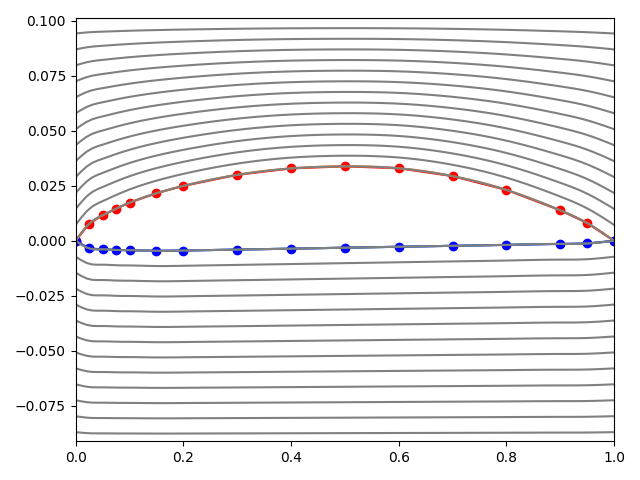
\includegraphics[width=0.5\linewidth]{res/air_flow.png}
\caption{The path of 30 particles in the space of an airfoil.}
\label{fig:airflow}
\end{figure}

In conclusion, the trajectories of air particles around the airfoil were succesfully drawn. The next step was to use these
trajectories to module the pressure map.

\subsection{Pressure Map }

All of the above amounts to plotting a pressure map around the wing, from which it is possible to deduce useful information about the airfoil's aerodynamic performance. Figure~\ref{fig:pressure_map} shows an example of pressure map.

\begin{figure}[H]
\centering
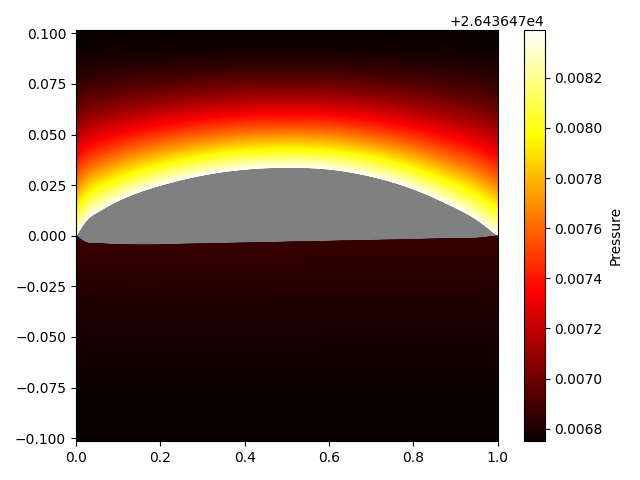
\includegraphics[width=0.5\linewidth]{res/pressure_map.png}
\caption{Pressure map example.}
\label{fig:pressure_map}
\end{figure}

The value of a pressure map lies in visually highlighting important information related to pressure around the airfoil being studied, processing it fluidly . It so appears that in the context of the mathematical modelisation chosen and the approximations made, air travels along a longer path right above the outer edge of the wing and decelerates at higher elevations, while air right below the inner edge of the wing seems to flow slower. Color coding facilitates the understanding of the map: darker areas express slower airflow rates, while lighter areas express faster airflow rates. The gray area corresponds to the wing itself, in which no flow naturally exists.

The function \verb|plot_pressure| generates the map by reading data from an input file, which contains the coordinates of the points tracing the airfoil's outer and inner edges. Cubic spline interpolation is then used to smooth out the wing's delimitations.

As described above, a parameter lambda is used to define the air particles flowing above and below the wing. For each of those, the airflow and line pressure are then calculated.

Finally, a pressure map such as Figure~\ref{fig:pressure_map} is ready to be plotted.
